\section{Programación Genética}

Programación Genética es un tipo de algoritmo evolutivo, inspirado en la evolución biológica y sus mecanismos principales. Antes de comentar las principales particularidades de Programación Genética explicaremos en que se basan los algoritmos evolutivos.

\subsection{Bases de algoritmos evolutivos}

Los algoritmos evolutivos son algoritmos que utilizan los mecanismos la evolución biológica, para intentar optimizar soluciones a un problema dado. Este tipo de algoritmos surgen tras diversas propuestas a finales de la década de 1950 \cite{historiaAlgoritmosEvolutivos} donde se proponen utilizar mecanismos basados en la biología para aplicarlos a máquinas de Turing. Tras estas propuestas, en la década de 1960 Hans-Joachim Bremermann desarrollo lo que sería la teoría de los algoritmos evolutivos.

\subsubsection{Funcionamiento de los algoritmos evolutivos}

La idea principal de este tipo de algoritmos es utilizar una población de individuos que serán soluciones al problema, de forma que aplicando ciertos mecanismos como la reproducción, mutación, recombinación, elitismo y selección la población evolucione hacia mejores soluciones. Estas soluciones se evaluarán utilizando una función objetivo que será la función a minimizar o maximizar.

El funcionamiento básico de este tipo de algoritmos es el siguiente:

\begin{enumerate}
	\item Generar una población inicial.
	\item Repetir hasta la condición de parada:
	\begin{enumerate}
		\item Evaluar la población actual para la función objetivo.
		\item Seleccionar los individuos que generarán la próxima generación.
		\item Aplicar la reproducción, mutación o recombinación de los individuos seleccionados, generando la población de hijos.
		\item Reemplazar la población de hijos por la población actual (con elitismo si así se quiere).
	\end{enumerate}
\end{enumerate}

Estos pasos generales son los que todo algoritmo evolutivo suele seguir, aunque existen muchas variantes. La condición de parada puede variar dependiendo de que se busque conseguir, puede ser, por ejemplo, que se realicen cierto número de evaluaciones de la población, o que se consiga cierto valor mínimo de la función objetivo.

Los distintos operadores de mutación, reproducción o recombinación no siempre son aplicados. Cada uno de estos eventos tendrá cierta probabilidad, de forma que el proceso será en parte aleatorio. Normalmente la recombinación o reproducción serán muy comunes, mientras que la mutación será más atípica.


\subsubsection{Modelos de población en algoritmos evolutivos}

También podemos hacer dos distinciones claras a la hora de como funcionan las poblaciones de este tipo de algoritmos:

\begin{itemize}
	\item Modelo de población generacional (figura \ref{fig:modelo_generacioal}): En este modelo la población es reemplazada por completo en cada iteración, de forma que se tienen que generar tantos hijos como elementos tiene la población.
	\item Modelo de población estacionario (figura \ref{fig:modelo_estacionario}): En este modelo solo se generan dos hijos, y esos dos hijos compiten por entrar en la población, reemplazando a los dos peores individuos de esta.
\end{itemize}

\begin{figure}[H]
    \centering
	  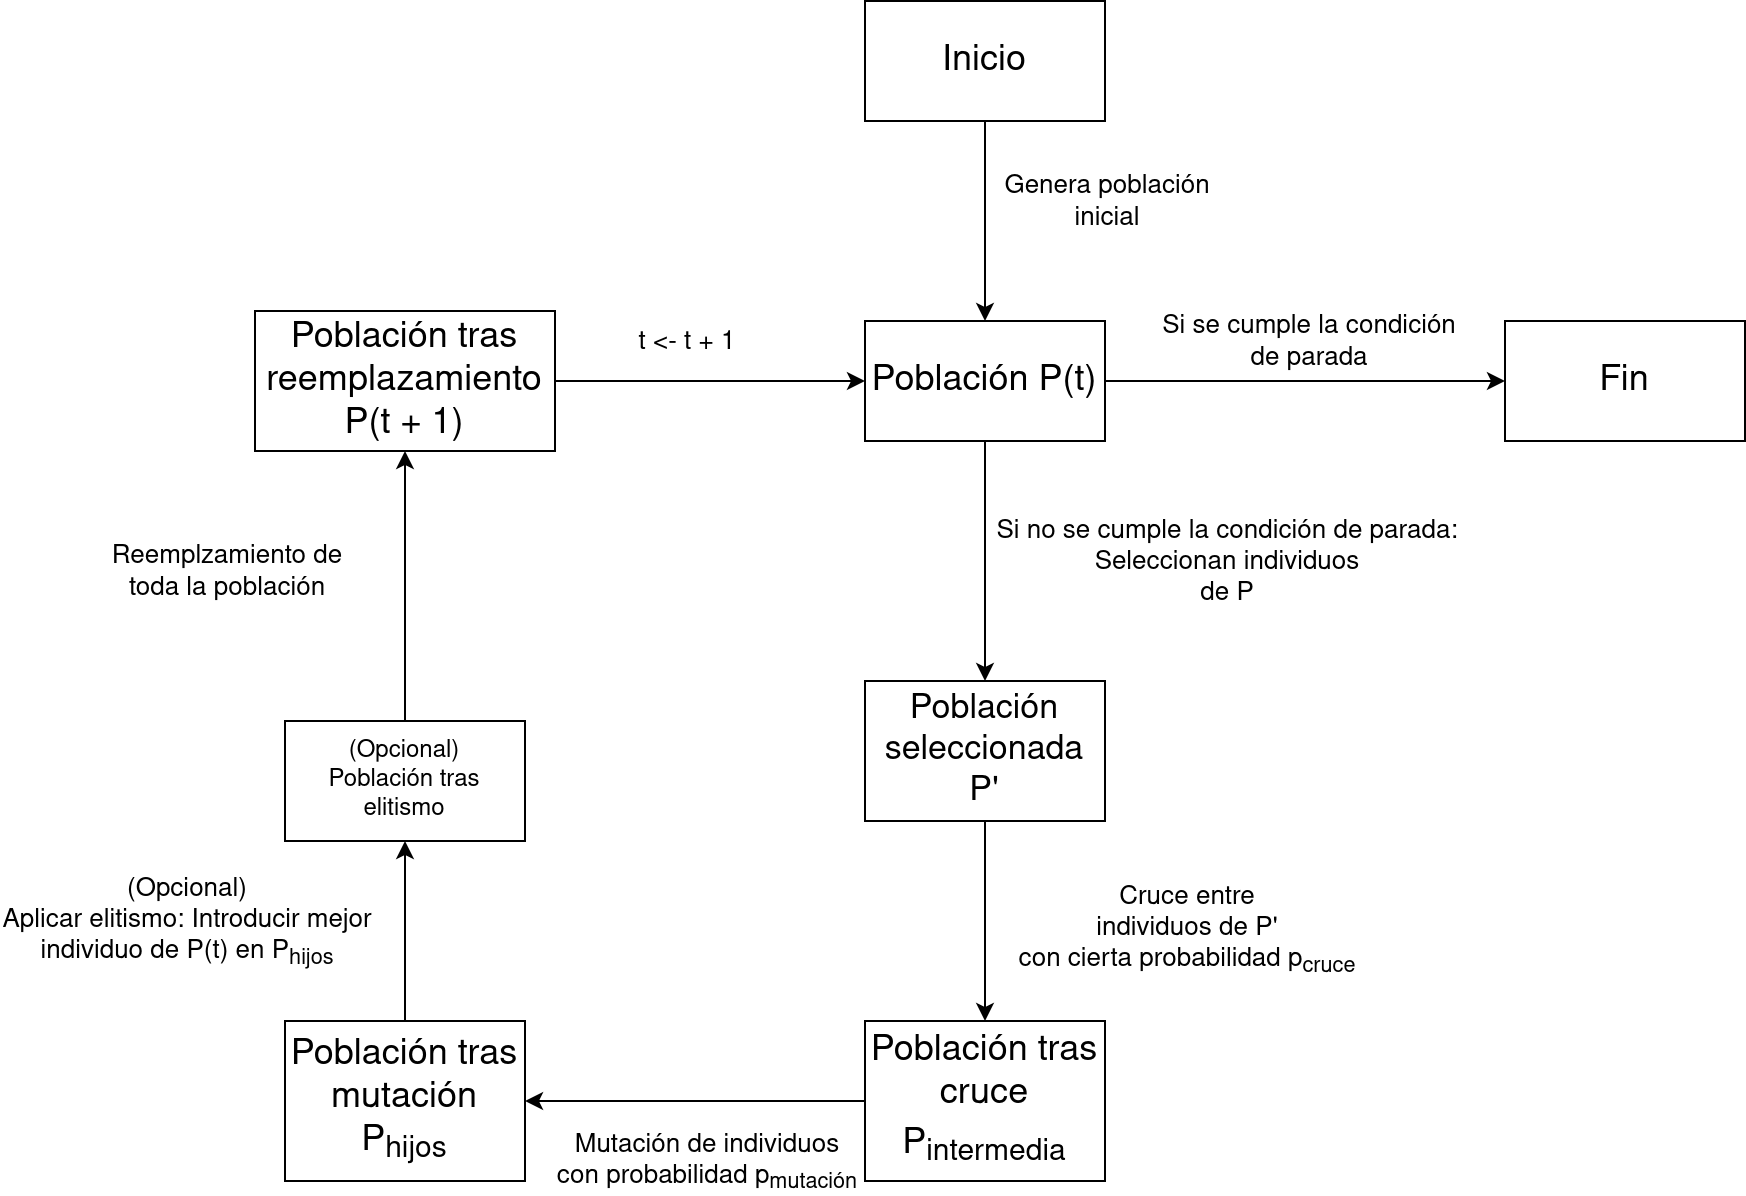
\includegraphics[width=\textwidth]{generacional.png}
    \caption{Esquema de un algoritmo evolutivo con un modelo generacional.}
	 \label{fig:modelo_generacioal}
\end{figure}

\begin{figure}[H]
    \centering
	  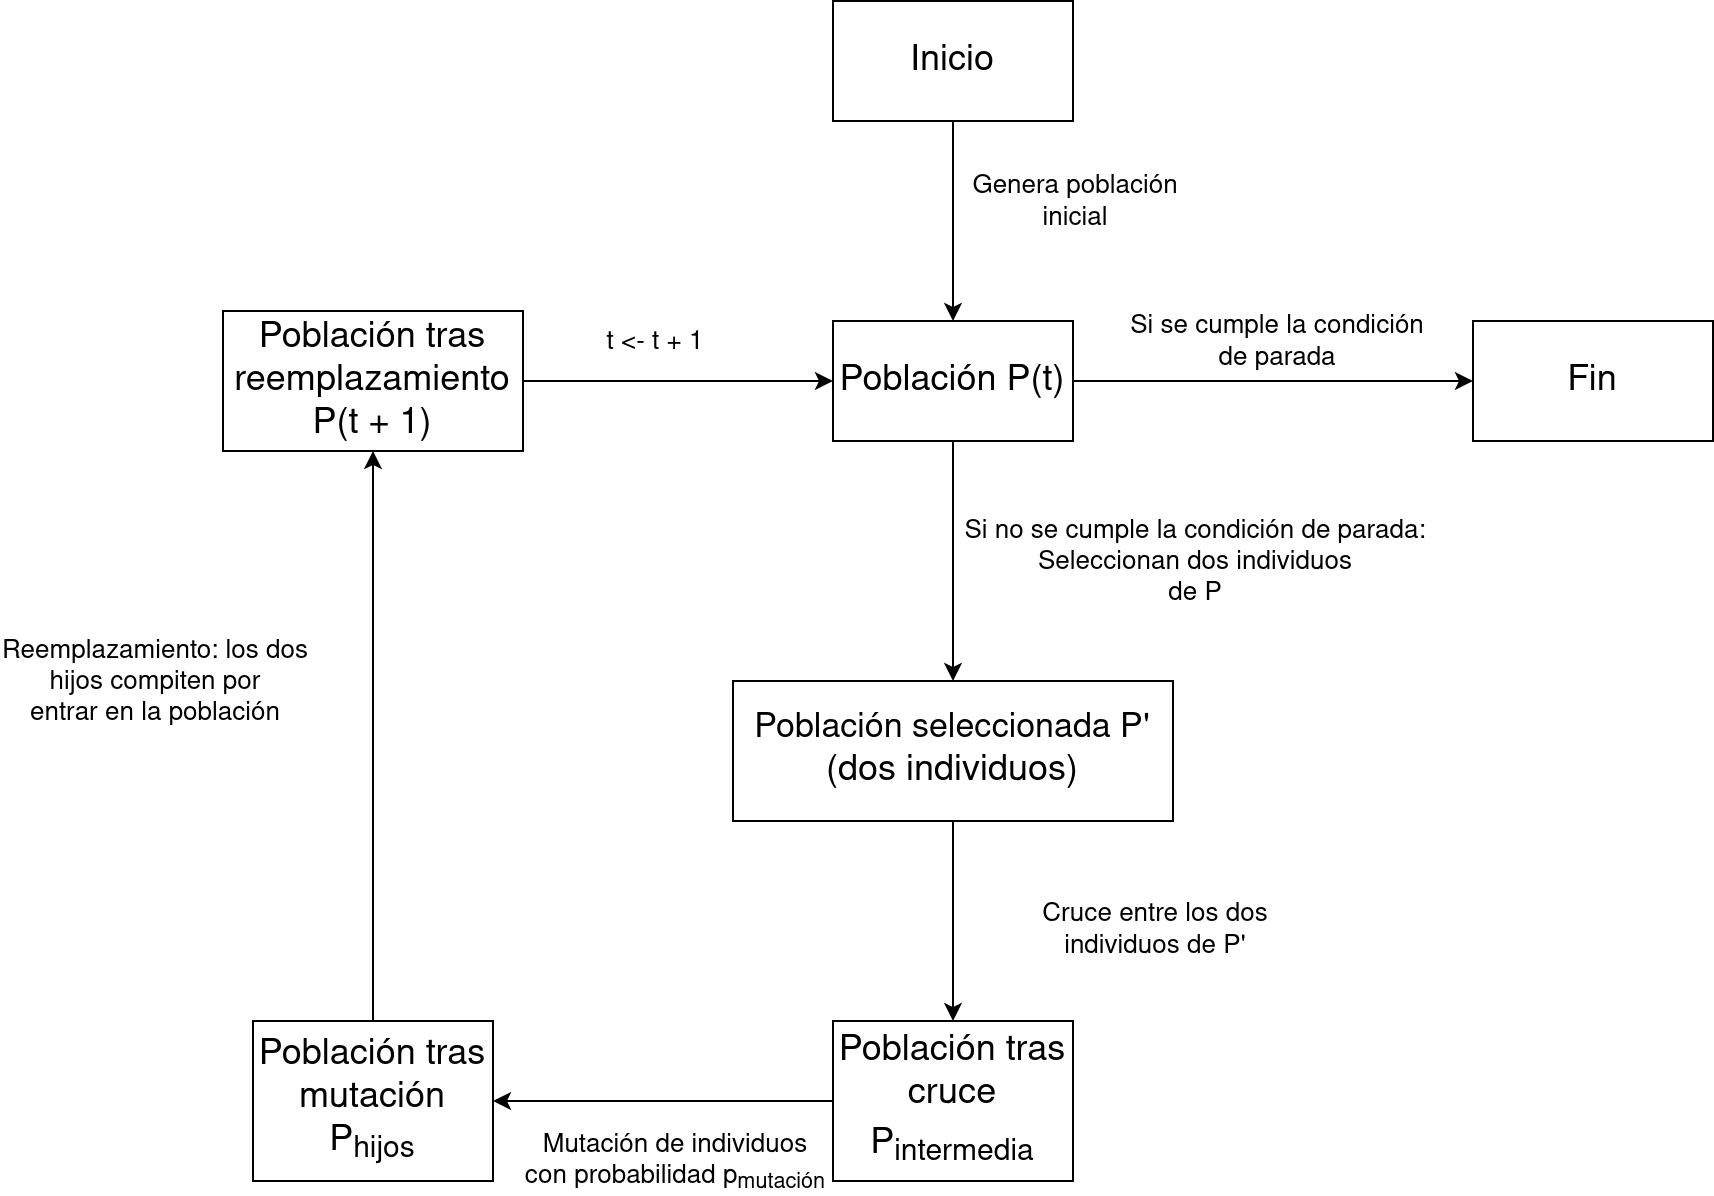
\includegraphics[width=\textwidth]{estacionario.png}
    \caption{Esquema de un algoritmo evolutivo con un modelo estacionario.}
	 \label{fig:modelo_estacionario}
\end{figure}


\subsubsection{Principales paradigmas de algoritmos evolutivos}

Existen cuatro enfoques básicos de algoritmos evolutivos.

\begin{enumerate}
	\item Estrategias de Evolución.
	\item Programación Evolutiva.
	\item Algoritmos Genéticos.
	\item Programación Genética.
\end{enumerate}

El primer enfoque, Estrategias de Evolución, es desarrollado por Hans-Paul Schwefel e Ingo Rechenberg a partir de 1964 y presentado en 1971 como su tesis doctoral \cite{estrategiasEvolucion}. En este trabajo se enfatiza en como los individuos de la población realizan sus cambios, haciendo un análisis más exhaustivo en como aplicar los cambios a los individuos, y no en su representación como tal.

El segundo enfoque, Programación Evolutiva, fue propuesto por Lawrence J. Fogel en 1966 \cite{programacionEvolutiva}, y es de los primeros trabajos donde se propone un algoritmos basado en algoritmos evolutivos y la teoría desarrollada por Bremermann.

El tercer enfoque, Algoritmos Genéticos, propuesto en 1975 por John Holland, de la Universidad de Michigan, en su libro publicado ese mismo año \cite{libroAlgoritmosGeneticos}. Este enfoque se basaba en dar a los elementos de la población una representación en cromosomas, de forma que se aplicaban operadores genéticos sobre dichos cromosomas para hacerlos evolucionar y mejorar su valor de la función objetivo.

El último enfoque, Programación Genética, es el que utilizaremos, y se explicará más en detalle en los siguientes apartados.


\subsection{Como funciona Programación Genética}

Programación Genética fue impulsada por John Koza a comienzos de la década de 1990 \cite{kozaGP}. Este enfoque de algoritmo evolutivo se basa en utilizar expresiones en forma de árbol como individuos de la población. Con esta representación en árbol se puede llegar a entrenar desde fórmulas matemáticas o lógicas, hasta programas escritos en C o cualquier otro lenguaje de programación cuya gramática se pueda expresar como un árbol.

\begin{figure}[H]
    \centering
	 \begin{subfigure}[b]{0.49\textwidth}
		 \centering
		 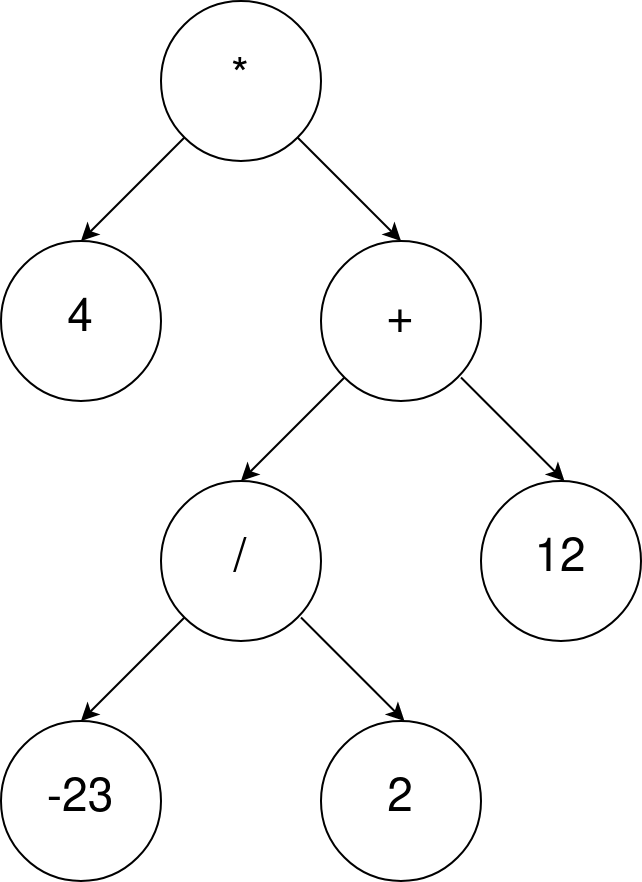
\includegraphics[width=0.5\textwidth]{arbol_exp_matematica.png}
		 \caption{Expresión matemática $4 \cdot ( (-23 / 2) + 12)$ representada como un árbol.}
		 \label{fig:exp_matematica}
	 \end{subfigure}
	 \begin{subfigure}[b]{0.49\textwidth}
		 \centering
		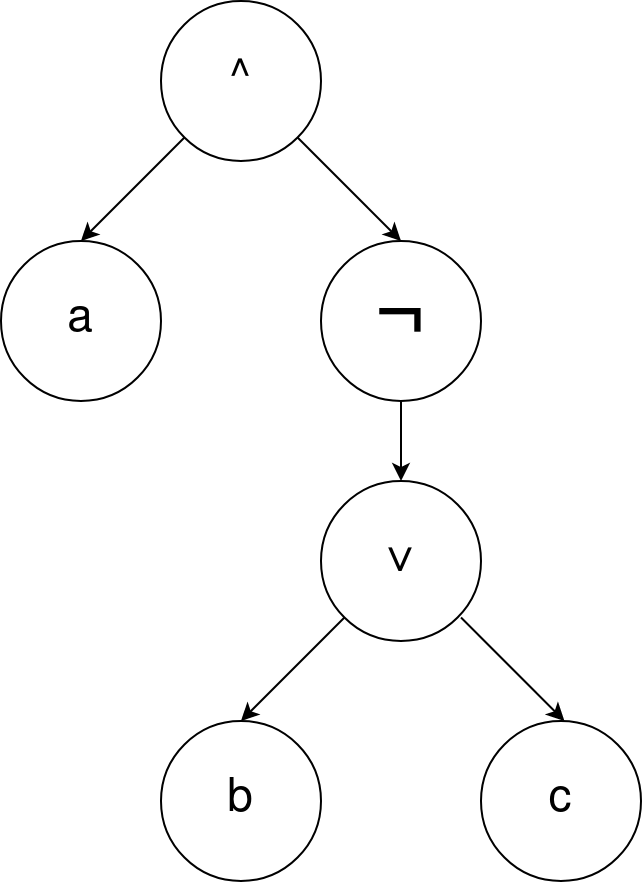
\includegraphics[width=0.5\textwidth]{arbol_exp_logica.png}
		\caption{Expresión lógica $ a \wedge (\neg (b \vee c) ) $ representada como un árbol.}
		\label{fig:exp_logica}
   \end{subfigure}
	\caption{Algunos ejemplos de expresiones representadas como árboles.}
	\label{fig:arbol_exp}
\end{figure}

Como podemos imaginar, estos árboles no son de un tamaño ni profundidad fijas, si no que el tamaño de los individuos será variable, a diferencia de los cromosomas utilizados en Algoritmos Genéticos.

También tenemos que tener en cuenta que en este caso evaluar la población requiere recorrer cada árbol por completo de forma recursiva, por lo que esto será una operación bastante costosa.

De cara a funcionar con expresiones en forma de árbol, los operadores de Programación Genética deben tener en cuenta esta estructura.

\subsection{Operadores de Programación Genética}

\subsubsection{Operador de cruce}

El operador de cruce de Programación Genética se trata de una recombinación de subárboles escogidos de forma aleatoria.

\begin{figure}[H]
    \centering
	 \begin{subfigure}[b]{\textwidth}
		 \centering
		 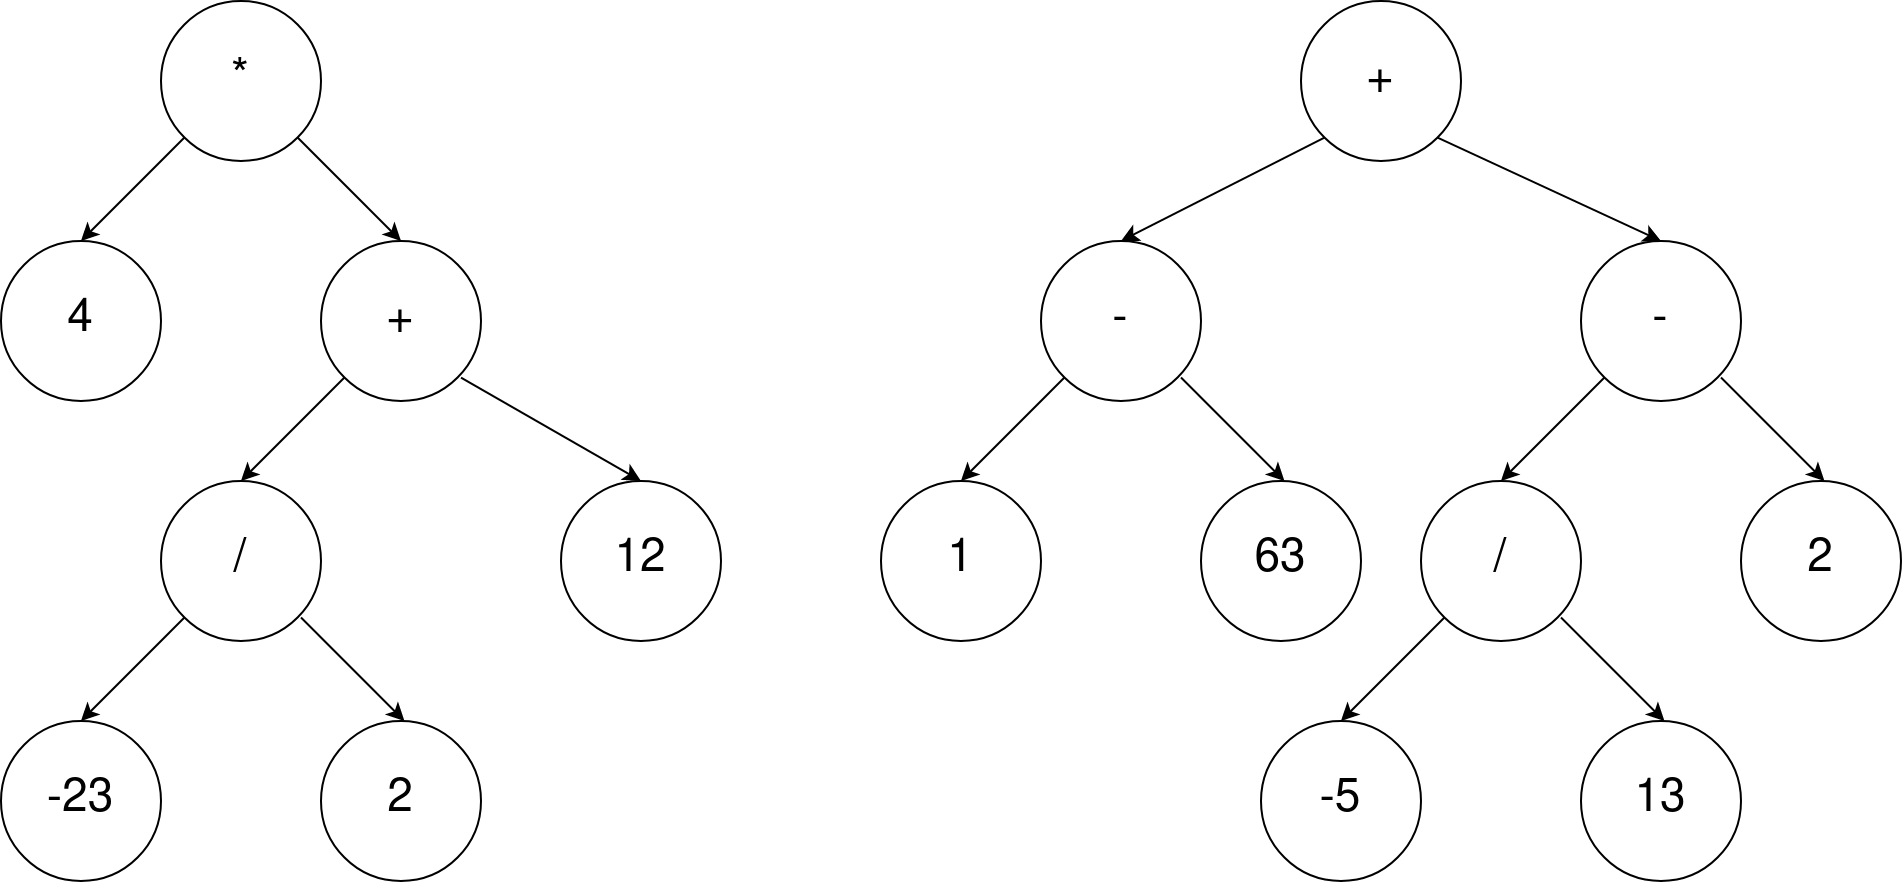
\includegraphics[width=0.5\textwidth]{cruce_GP.png}
		 \caption{Dos expresiones a cruzar.}
		 \label{fig:cruce_GP}
	 \end{subfigure}

	\begin{subfigure}[b]{\textwidth}
		 \centering
		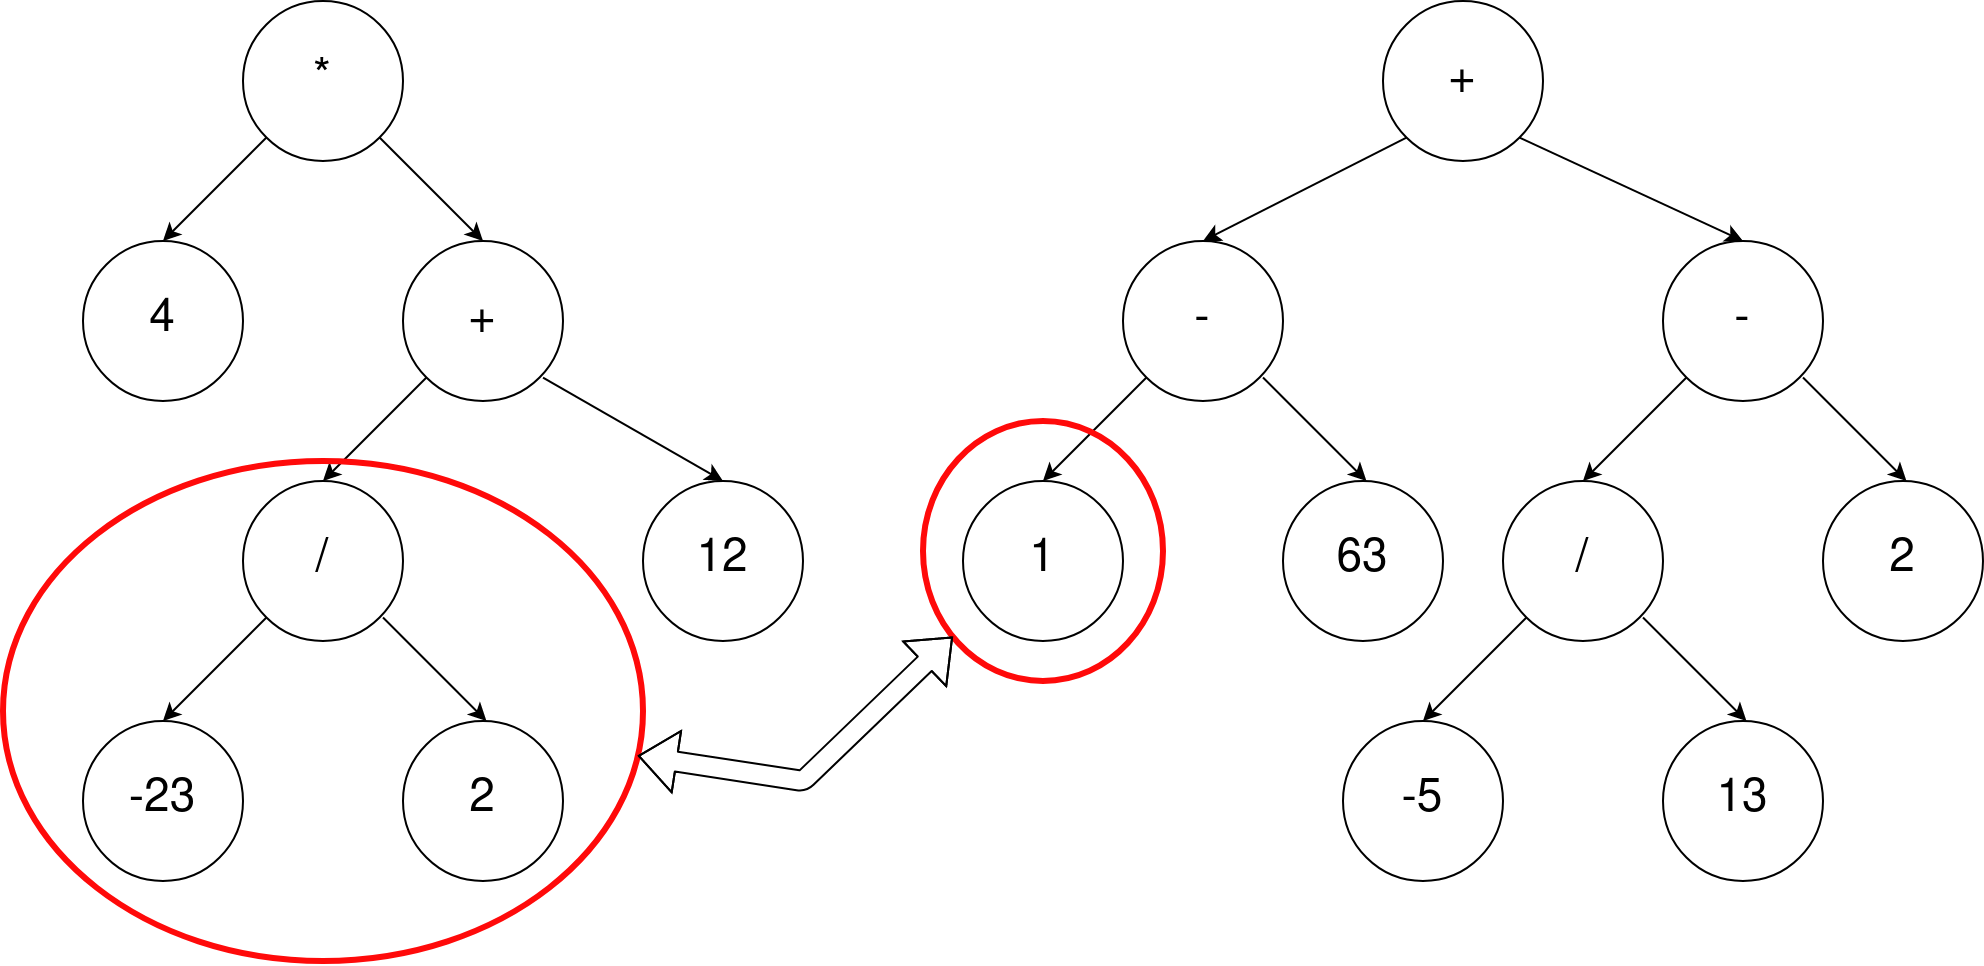
\includegraphics[width=0.5\textwidth]{cruce_GP_seleccion.png}
		\caption{Selección aleatoria de los subárboles a cruzar.}
		\label{fig:cruce_GP_seleccion}
   \end{subfigure}

	\begin{subfigure}[b]{\textwidth}
		\centering
	  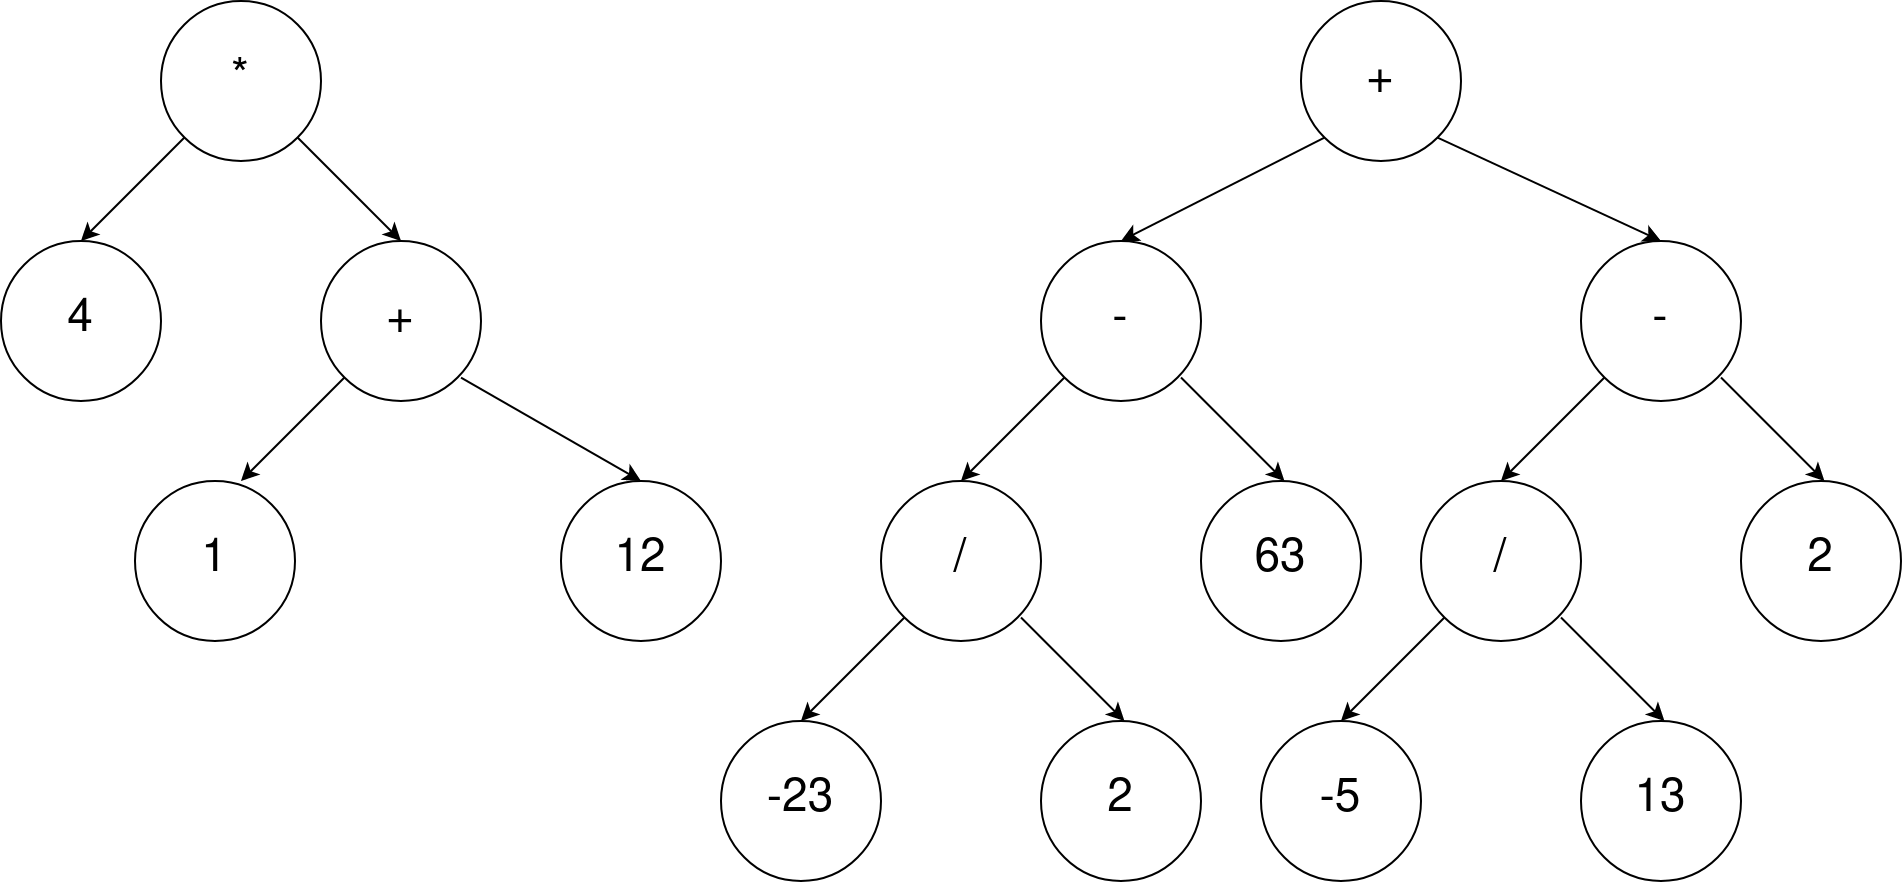
\includegraphics[width=0.5\textwidth]{cruce_GP_final.png}
	  \caption{Expresiones tras realizar el cruce.}
	  \label{fig:cruce_GP_final}
   \end{subfigure}

	\caption{Ejemplo del operador de cruce en dos árboles.}
	\label{fig:ej_cruce_GP}
\end{figure}

Como vemos en la figura \ref{fig:ej_cruce_GP}, se trata simplemente de escoger dos puntos al azar en el árbol e intercambiar los respectivos subárboles, aunque esto puede acarrear problemas ya que podríamos llegar a tener árboles excesivamente grandes.

\subsubsection{Operador de mutación}

El operador de mutación puede tener dos comportamientos. Este operador escogerá un punto al azar del árbol, y puede:

\begin{enumerate}
	\item Reemplazar de forma aleatoria el valor del nodo actual (siempre por un nodo del mismo tipo) (figura \ref{fig:mutacion_suave}).
	\item Reemplazar el subárbol a partir del punto escogido (figura \ref{fig:mutacion_fuerte}).
\end{enumerate}

\begin{figure}[H]
    \centering
	 \begin{subfigure}[b]{0.49\textwidth}
		 \centering
		 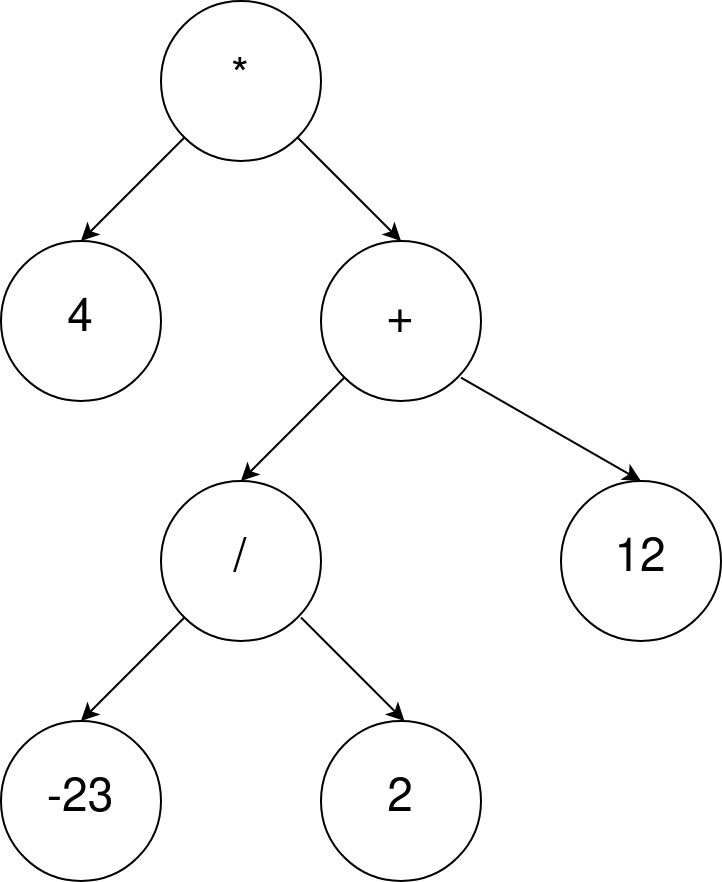
\includegraphics[width=0.5\textwidth]{arbol_mutar.png}
		 \caption{Expresión a mutar.}
		 \label{fig:arbol_mutar}
	 \end{subfigure}
	\begin{subfigure}[b]{0.49\textwidth}
		 \centering
		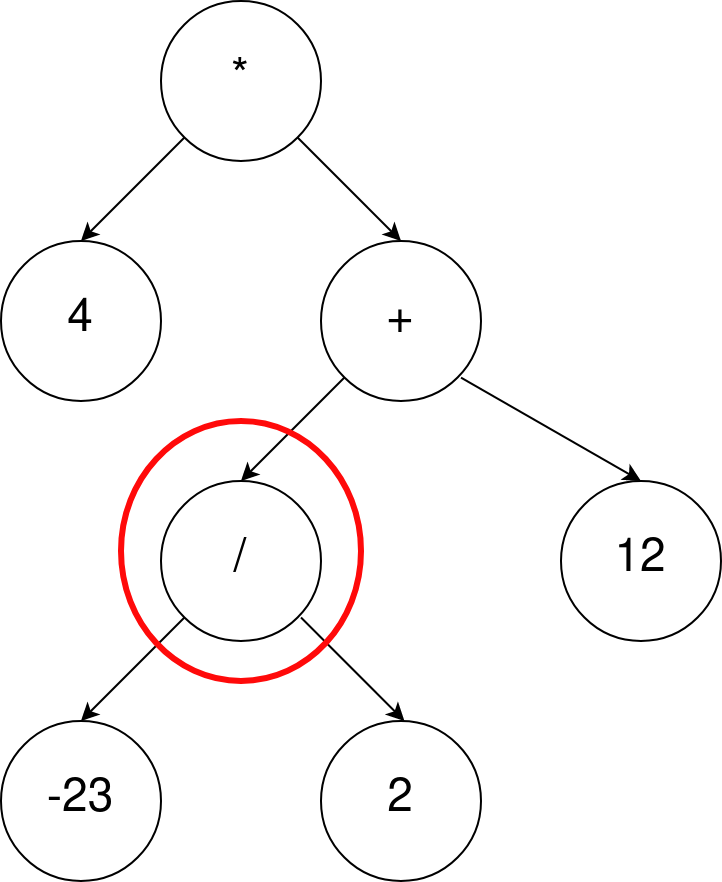
\includegraphics[width=0.5\textwidth]{punto_mutacion.png}
		\caption{Selección aleatoria del punto a mutar.}
		\label{fig:punto_mutacion}
   \end{subfigure}

	\begin{subfigure}[b]{0.49\textwidth}
		\centering
	  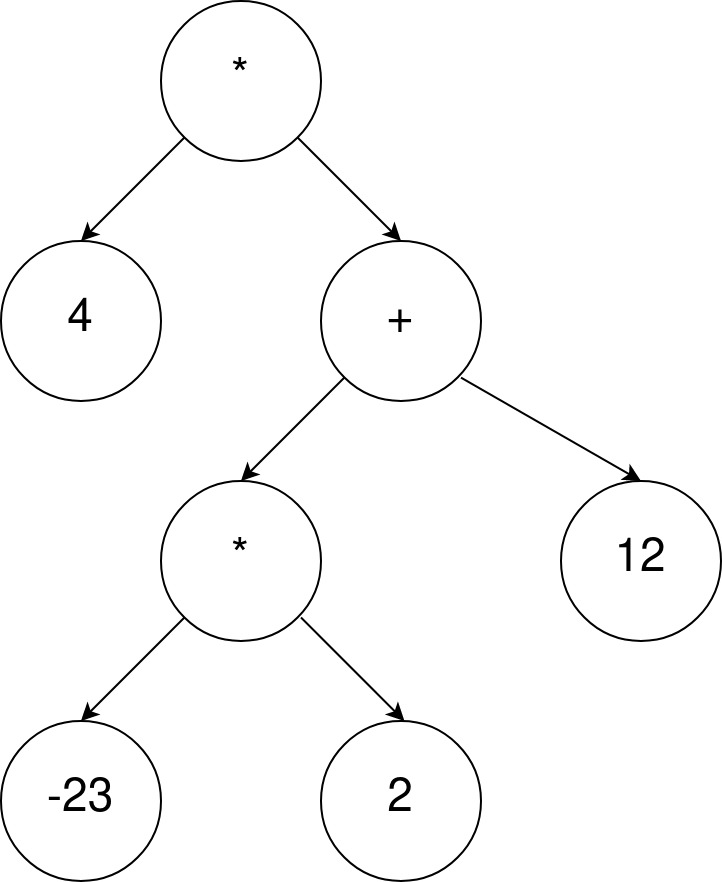
\includegraphics[width=0.5\textwidth]{mutacion_suave.png}
	  \caption{Expresiones tras realizar la mutación de tipo 1.}
	  \label{fig:mutacion_suave}
   \end{subfigure}
	\begin{subfigure}[b]{0.49\textwidth}
		\centering
	  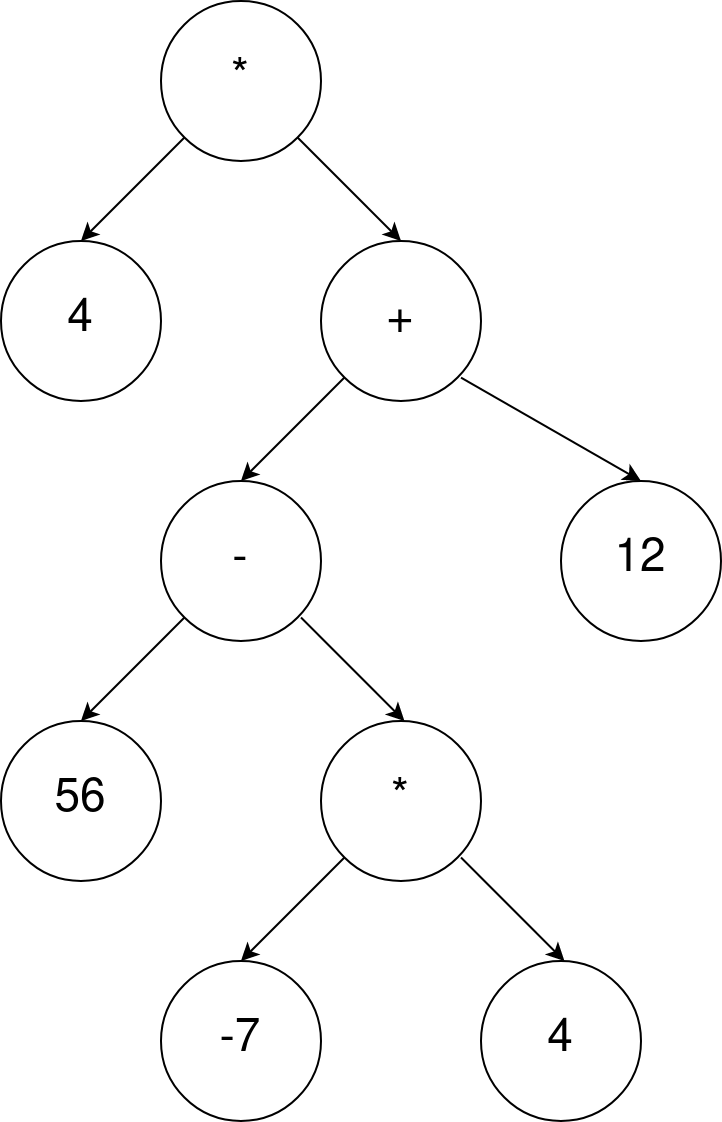
\includegraphics[width=0.5\textwidth]{mutacion_fuerte.png}
	  \caption{Expresiones tras realizar la mutación de tipo 2.}
	  \label{fig:mutacion_fuerte}
	\end{subfigure}

	\caption{Ejemplo del operador de mutación sobre un individuo.}
	\label{fig:ej_mutacion_GP}
\end{figure}

En este caso el segundo tipo de mutación nos ofrece una mayor diversidad en las expresiones y por eso es la que se suele utilizar, aunque cabe mencionar que el propio operador de cruce ya añade suficiente diversidad y por este motivo la mutación no es tan importante en Programación Genética.

\subsection{Problemas de Programación Genética}

\subsubsection{Sobreajuste en el tamaño de los árboles}

\subsubsection{Aprendizaje de constantes}


\subsection{Mi implementación de Programación Genética}

\subsection{Resultados}

\subsection{Problemas de Programación Genética}
